%----------------------------------------------------------------------------------------------------------
% Slide 52

\begin{frame}
  \myheading{Module 6.8 : Singular Value Decomposition }
\end{frame}

\begin{frame}
  \begin{center}
    \textit{Let us get some more perspective on eigen vectors before moving ahead}
  \end{center}
\end{frame}

%----------------------------------------------------------------------------------------------------------
% Slide 53
\begin{frame}
  \begin{overlayarea}{\textwidth}{\textheight}
    \begin{itemize}\justifying
      \item<1-> Let $v_1,v_2,\cdots,v_n$ be the eigen vectors of $A$ and let $\lambda_1,\lambda_2,\cdots,\lambda_n$ be corresponding eigen values
            \begin{equation*}
              Av_1 = \lambda_1v_1, Av_2 = \lambda_2v_2,\cdots,Av_n = \lambda_nv_n
            \end{equation*}
      \item<2-> If a vector $x$ in $\mathbb{R}^n$ is represented using $v_1,v_2,\cdots,v_n$ as basis then
            \begin{align*}
              \begin{split}
                x &= \sum_{i=1}^{n} \alpha_i v_i \\
                \onslide<3->{\text{Now}, Ax &= \sum_{i=1}^{n} \alpha_i Av_i = \sum_{i=1}^{n} \alpha_i \lambda_i v_i }
              \end{split}
            \end{align*}
      \item<4-> The matrix multiplication reduces to a scalar multiplication if the eigen vectors of $A$ are used as a basis.
    \end{itemize}
  \end{overlayarea}
\end{frame}

%----------------------------------------------------------------------------------------------------------
% Slide 54
\begin{frame}
  \begin{overlayarea}{\textwidth}{\textheight}
    \vspace{0.9cm}
    \begin{itemize}\justifying
      \item<1-> So far all the discussion was centered around square matrices ($A \in \mathbb{R}^{n \times n}$)
      \item<2-> What about rectangular matrices $A \in \mathbb{R}^{m \times n}$? Can they have eigen vectors?
      \item<3-> Is it possible to have $A_{m \times n} x_{n \times 1} = x_{n \times 1}$? \onslide<4->{Not possible !}
      \item<5-> The result of $A_{m \times n} x_{n \times 1}$ is a vector belonging to $\mathbb{R}^m$ (whereas $x \in \mathbb{R}^n$)
      \item<6-> So do we miss out on the advantage that a basis of eigen vectors provides for square matrices (i.e. converting matrix multiplications into scalar multiplications)?
      \item<7-> We will see the answer to this question over the next few slides
    \end{itemize}
  \end{overlayarea}
\end{frame}

%----------------------------------------------------------------------------------------------------------
% Slide 55
\begin{frame}[shrink=5]
  \begin{overlayarea}{\textwidth}{\textheight}
    \vspace{-0.2cm}
    {\small
      \begin{itemize}\justifying
        \item<1-> Note that matrix $A_{m \times n}$ provides a transformation $\mathbb{R}^n \rightarrow \mathbb{R}^m$
        \item<2-> What if we could have pairs of vectors $(v_1,u_1),(v_2,u_2),\cdots,(v_k,u_k)$ such that $v_i \in \mathbb{R}^n$, $u_i \in \mathbb{R}^m$ and $Av_i=\sigma_i u_i$
        \item<3-> Further let's assume that $v_1,\cdots,v_k,\cdots,v_n$ are orthogonal \& thus form a basis $V$ in $\mathbb{R}^n$
        \item<4-> Similarly let's assume that $u_1,\cdots,u_k,\cdots,u_m$ are orthogonal \& thus form a basis $U$ in $\mathbb{R}^m$
        \item<5-> Now what if every vector $x \in \mathbb{R}^n$ is represented using the basis $V$
              \begin{align*}
                \begin{split}
                  \onslide<6->{    x &= \sum_{i=1}^{k} \alpha_i v_i \qquad \qquad [\textnormal{note we are using \textit{k} instead of \textit{n} ; will clarify this in a minute}]} \\
                  \onslide<7->{   Ax &= \sum_{i=1}^{k} \alpha_i A v_i } \\
                  \onslide<8->{       &= \sum_{i=1}^{k} \alpha_i \sigma_i u_i}
                \end{split}
              \end{align*}
        \item<9-> Once again the matrix multiplication reduces to a scalar multiplication
      \end{itemize}
    }
  \end{overlayarea}
\end{frame}

%----------------------------------------------------------------------------------------------------------
% Slide 56
\begin{frame}
  \begin{center}
    Let's look at a geometric interpretation of this
  \end{center}
\end{frame}

%----------------------------------------------------------------------------------------------------------
% Slide 57
\begin{frame}
  \begin{overlayarea}{\textwidth}{\textheight}
    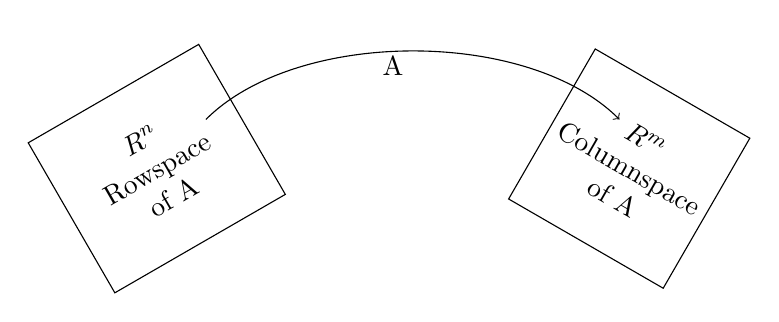
\begin{tikzpicture}<1->[scale=0.75]
  \node[rectangle,draw,rotate=30,minimum height=22mm,minimum width=25mm,align=center] at (2,0) {$\mathbb{R}^n$ \\ Rowspace \\ of A};
  \node[rectangle,draw,rotate=-30,minimum height=22mm,align=center] at (8,0) {$\mathbb{R}^m$ \\ Columnspace \\ of A};
  \node (1) at (2.5,0.5) {};
  \node (2) at (8,0.5) {};
  \node at (5,1.3){A};
  \draw (1) edge[looseness=0.8,->] (2);
\end{tikzpicture}

    {\small
    \onslide<1->{
      \hspace{0.1cm}dim=$k$=rank(A) \hspace{4cm} dim=$k$=rank(A)} \\
    %\vspace{0.7cm}
    \begin{itemize}\justifying
      \item \onslide<2->{$\mathbb{R}^n$ - Space of all vectors which can multiply with $A$ to give $Ax$ [ this is the space of inputs of the function]}\\
      \item \onslide<3->{$\mathbb{R}^m$ - Space of all vectors which are outputs of the function $Ax$} \\
      \item \onslide<4->{We are interested in finding a basis $U$, $V$ such that} \\
            \begin{itemize}\justifying
              \item \onslide<5->{$V$ - basis for inputs }\\
              \item \onslide<6->{$U$ - basis for outputs }\\
            \end{itemize}
      \item \onslide<7>{such that if the inputs and outputs are represented using this basis then the operation $Ax$ reduces to a scalar operation}
    \end{itemize}
    }
  \end{overlayarea}
\end{frame}

%----------------------------------------------------------------------------------------------------------
% Slide 58
\begin{frame}
  \begin{overlayarea}{\textwidth}{\textheight}
    \vspace{0.9cm}
    \begin{itemize}\justifying
      \item<1-> What do we mean by saying that dimension of rowspace is $k$? If $x \in \mathbb{R}^n$ then why is the dimension not $n$.
      \item<2-> It means that of all the possible vectors in $\mathbb{R}^n$ only a subspace of vectors lying in $\mathbb{R}^k$ can act as inputs to $Ax$ and produce a non-zero output. The remaining vectors in $\mathbb{R}^{n-k}$ will produce a zero output
      \item<3-> Hence we need only $k$ dimensions to represent $x$
            \begin{equation*}
              x = \sum_{i=1}^{k}\alpha_iv_i
            \end{equation*}
    \end{itemize}
  \end{overlayarea}
\end{frame}

%----------------------------------------------------------------------------------------------------------
% Slide 59
\begin{frame}
  \begin{overlayarea}{\textwidth}{\textheight}
    \begin{itemize}\justifying
      \item<1-> Let's look at a way of writing this as a matrix operation
            \begin{equation*}
              Av_1 = \sigma_1u_1, Av_2 = \sigma_2u_2,\cdots,Av_k = \sigma_k u_k
            \end{equation*}
            \begin{equation*}
              A_{m \times n} V_{n \times k} = U_{m \times k} \underbrace{\Sigma_{k \times k}}_{\textnormal{diagonal matrix}}
            \end{equation*}
      \item<2-> If we have $k$ orthogonal vectors ($V_{n \times k}$) then using Gram Schmidt orthogonalization, we can find $n-k$ more orthogonal vectors to complete the basis for $\mathbb{R}^n$ [We can do the same for U]
            \begin{equation*}
              A_{m \times n} V_{n \times n} = U_{m \times m} \Sigma_{m \times n}
            \end{equation*}
            \begin{equation*}
              U^T AV = \Sigma \qquad [U^{-1}=U^T] \qquad A = U\Sigma V^T \qquad [V^{-1}=V^T]
            \end{equation*}
      \item<3-> $\Sigma$ is a diagonal matrix with only the first $k$ diagonal elements as non-zero
      \item<4-> Now the question is how do we find $V$, $U$ and $\Sigma$
    \end{itemize}
  \end{overlayarea}
\end{frame}

%----------------------------------------------------------------------------------------------------------
% Slide 60
\begin{frame}
  \begin{overlayarea}{\textwidth}{\textheight}
    \begin{itemize}\justifying
      \item<1-> Suppose $V$, $U$ and $\Sigma$ exist, then
            \begin{align*}
              \begin{split}
                \onslide<2->{    A^T A &= (U \Sigma V^T)^T (U \Sigma V^T) }\\
                \onslide<3->{          &= V \Sigma^T U^T U \Sigma V^T }\\
                \onslide<4->{    A^T A &= V \Sigma^2 V^T }
              \end{split}
            \end{align*}
      \item<5-> What does this look like?\onslide<6->{ Eigen Value decomposition of $A^T A$}
      \item<7-> Similarly we can show that
            \begin{equation*}
              A A^T = U \Sigma^2 U^T
            \end{equation*}
      \item<8-> Thus $U$ and $V$ are the eigen vectors of $AA^T$ and $A^T A$ respectively and $\Sigma^2 = \Lambda$ where $\Lambda$ is the diagonal matrix containing eigen values of $A^T A$
    \end{itemize}
  \end{overlayarea}
\end{frame}

%----------------------------------------------------------------------------------------------------------
% Slide 61
\begin{frame}
  \begin{overlayarea}{\textwidth}{\textheight}
    \onslide<1->{
      \begin{align*}
        \begin{split}
          \begin{bmatrix}
             &  &   &  & \\
             &  &   &  & \\
             &  & A &  & \\
             &  &   &  &
          \end{bmatrix}_{m \times n} &= \begin{bmatrix}
            \uparrow   & \cdots & \uparrow   \\
                       &        &            \\
            u_1        & \cdots & u_k        \\
            \downarrow & \cdots & \downarrow
          \end{bmatrix}_{m \times k}\begin{bmatrix}
            \sigma_1 &        &          \\
                     & \ddots &          \\
                     &        & \sigma_k
          \end{bmatrix}_{k \times k}\begin{bmatrix}
            \leftarrow & v_1    & \rightarrow \\
                       & \vdots &             \\
            \leftarrow & v_k    & \rightarrow
          \end{bmatrix}_{k \times n}
        \end{split}            \\
         & = \sum_{i=1}^{k} \sigma_i u_i v_i^T
      \end{align*}
    }
    \vspace{-0.5cm}
    \onslide<2->{ \begin{block}{Theorem:}
        $\sigma_1 u_1 v_1^T$ is the best rank-1 approximation of the matrix $A$. $\sum_{i=1}^{2} \sigma_i u_i v_i^T$ is the best rank-2 approximation of matrix $A$.
        In general, $\sum_{i=1}^{k} \sigma_i u_i v_i^T$ is the best rank-k approximation of matrix $A$. In other words, the solution to
        \begin{align*}
          \begin{split}
            \min \left \| A - B \right \|_F^2 \quad \textnormal{is given by :} \\
            B =& U_{.,k} \Sigma_{k,k} V_{k,.}^T \quad (\textnormal{minimizes reconstruction error of A})
          \end{split}
        \end{align*}
      \end{block}
    }
  \end{overlayarea}
\end{frame}

%----------------------------------------------------------------------------------------------------------
% Slide 62
\begin{frame}
  \begin{center}
    \begin{align*}
      \begin{split}
        \onslide<1->{   \sigma_i &= \sqrt{\lambda_i} = \textnormal{singular value of A}} \\
        \onslide<2->{   U &= \textnormal{left singular matrix of A}} \\
        \onslide<3->{   V &= \textnormal{right singular matrix of A}}
      \end{split}
    \end{align*}
  \end{center}
\end{frame}